%-----------------------------------------------------------------------------%
\chapter{\babLima}
\label{bab:5}
Setelah melakukan implementasi metodologi dalam bentuk program, dilakukan beberapa eksperimen dengan tujuan menganalisis fitur-fitur yang digunakan untuk proses \reranking{}. Pada \bab{}~\ref{bab:5} akan dibahas hasil eksperimen dan analisisnya. \subbab{}~\ref{subbab:5:hasil dan kajian base retriever} mengandung analisis awal yang dilakukan untuk melakukan seleksi kandidat \base{} \retriever{} yang akan digunakan pada skenario-skenario selanjutnya. Setelah melakukan seleksi, akan dijalankan beberapa skenario eksperimen yang akan dijelaskan pada \subbab{}~\ref{subbab:5:Skenario Eksperimen}. Kemudian, \subbab{}~\ref{subbab:5:Hasil Eksperimen} menyampaikan hasil eksperimen yang telah dijalankan dalam bentuk grafik, tabel, dan analisis. Terakhir, terdapat \subbab{}~\ref{subbab:5:Rangkuman Hasil Eksperimen} yang merangkum seluruh hasil analisis yang telah dilakukan pada \subbab{} sebelumnya.
%-----------------------------------------------------------------------------%





%-----------------------------------------------------------------------------%
\section{Skenario Eksperimen}
\label{subbab:5:Skenario Eksperimen}
Setelah melakukan seleksi 5 model yang akan digunakan sebagai \base{} \retriever{}, dibangun sebuah sistem \cascaded{} \ir{} untuk masing-masing model tersebut. Sistem \ir{} sejumlah 5 inilah yang akan digunakan pada beberapa skenario penelitian untuk analisis fitur dan efektivitas. Pada \subbab{}~\ref{subbab:5::Analisis Bobot Fitur} dijelaskan mengenai skenario analisis \feature{} \importance{} menggunakan \fcv{}. Kemudian, \subbab{}~\ref{subbab:5::Pengaruh Cut-off} membahas pengaruh \cutoff{} pada efektivitas proses \reranking{} dengan \reranker{} berbasis fitur.
%-----------------------------------------------------------------------------%





%-----------------------------------------------------------------------------%
\subsection{Analisis Bobot Fitur}
\label{subbab:5::Analisis Bobot Fitur}
Pada skenario ini, akan diuji lima sistem \cascaded{} \ir{} yang terdiri dari dua tahap \ranking{}. Tahap pertama akan menggunakan salah satu dari lima model yang telah dipilih pada \subbab{}~\ref{subbab:5:hasil dan kajian base retriever}. Berdasarkan hasil \ranking{} awal, semua fitur yang diusulkan dalam \subbab{}~\ref{subbab:3:Usulan Fitur} akan diekstraksi dan kemudian diteruskan ke tahap kedua yang akan menggunakan \lambdamart{} untuk proses \ranking{} lanjutan.

Skenario ini akan dijalankan dengan metode \fcv{}. Metode ini membagi data menjadi lima bagian yang sama, di mana setiap bagian secara bergantian digunakan sebagai data uji sementara bagian lainnya digunakan sebagai data pelatihan. Hal ini memastikan bahwa \reranker{} dilatih menggunakan data yang terpisah dari data percobaan \retrieval{} di setiap \textit{fold}-nya, sehingga setiap bagian data mendapatkan giliran untuk dipakai sebagai data percobaan.

Selain menguji lima sistem utama, skenario ini juga akan menyertakan model \base{} \retriever{} sebagai pembanding untuk mengukur efektivitas proses \retrieval{}. Dengan cara ini, akan terlihat sejauh mana peningkatan kinerja yang dihasilkan oleh sistem \cascaded{} \ir{} dibandingkan dengan model dasar.
%-----------------------------------------------------------------------------%





%-----------------------------------------------------------------------------%
\subsection{Pengaruh \Cutoff{}}
\label{subbab:5::Pengaruh Cut-off}
Dalam skenario ini, peneliti bertujuan untuk menyelidiki pengaruh nilai \cutoff{} terhadap efektivitas proses \retrieval{} dalam sistem \cascaded{} \ir{}. Eksperimen yang dilakukan mengikuti metodologi yang serupa dengan skenario sebelumnya, namun dengan perbedaan penting yaitu eksperimen yang dilakukan hanya menggunakan satu kali pembagian data untuk pelatihan dan percobaan. Dengan menetapkan pembagian data sebanyak satu kali, pengamatan yang dilakukan lebih spesifik terkait pengaruh nilai \cutoff{} tanpa melibatkan variasi pembagian data yang berbeda-beda.

Nilai \cutoff{} yang dimaksud mengacu pada jumlah dokumen yang dipilih untuk diteruskan dari tahap \ranking{} pertama ke tahap kedua. Peneliti memiliki hipotesis bahwa terdapat korelasi positif antara nilai \cutoff{} dan efektivitas \retrieval{}. Artinya, semakin tinggi nilai \cutoff{}, diharapkan semakin tinggi pula efektivitas proses \retrieval{} karena lebih banyak dokumen yang akan dipertimbangkan pada tahap \ranking{} kedua dengan model \lambdamart{}. Untuk menguji hipotesis ini, eksperimen ditetapkan dengan menggunakan beberapa nilai \cutoff{} yang berbeda dan mengukur efektivitas pada setiap nilai tersebut.Hasil dari eksperimen ini akan dianalisis untuk melihat apakah peningkatan nilai \cutoff{} memang berkontribusi terhadap peningkatan efektivitas \retrieval{}, serta untuk menentukan \cutoff{} optimal yang memberikan keseimbangan terbaik antara jumlah dokumen yang diproses dan efektivitas hasil akhir.
%-----------------------------------------------------------------------------%





%-----------------------------------------------------------------------------%
\section{Hasil dan Kajian \textit{Base Retriever}}
\label{subbab:5:hasil dan kajian base retriever}
Sebelum melakukan skenario yang telah dirancang, pertama-tama dilakukan kajian beberapa \base{} \retriever{} seperti yang sudah disinggung pada \subbab{}~\ref{subbab:3:Kajian Base Retrieval}. Kajian dilakukan menggunakan hasil dari percobaan \retrieval{} menggunakan hanya \base{} \retriever{} untuk mengembalikan dokumen relevan. Percobaan tersebut dilakukan dengan memanfaatkan keseluruhan data \training{} dan tidak menggunakan pemisahan data validasi karena tidak diperlukannya pelatihan terlebih dahulu untuk model-model tersebut. Setelah dilakukan percobaan \retrieval{}, beberapa metrik dihitung sebagai alat ukur kinerja dari model. Berdasarkan hasil percobaan yang didapat pada \tabel{}~\ref{tabel:5:base retriever}, akan dilakukan seleksi beberapa \base{} \retriever{} yang layak untuk dibangun menjadi sistem \ir{}.
\begin{table}
    \centering
    \caption{Kinerja \base{} \retriever{} pada data \training{}}
    \label{tabel:5:base retriever}
    \resizebox{\textwidth}{!}{%
        \begin{tabular}{lrrrrrrrrr}
	\toprule
	name & R@3 & R@5 & R@10 & recip\_rank & P@3 & P@5 & P@10 & map & nDCG@5 \\
	\midrule
	InL2 & \textbf{0,6281} & \textbf{0,6836} & 0,7403 & 0,6284 & \underline{0,2373} & \textbf{0,1566} & 0,0861 & 0,5912 & \underline{0,6115} \\
	DLH13 & \underline{0,6277} & 0,6812 & 0,7374 & \textbf{0,6311} & \textbf{0,2376} & \underline{0,1564} & 0,0862 & \textbf{0,5945} & \textbf{0,6130} \\
	DFR\_BM25 & 0,6262 & \underline{0,6823} & \textbf{0,7443} & 0,6268 & 0,2359 & 0,1560 & \textbf{0,0867} & 0,5891 & 0,6093 \\
	BM25 & 0,6257 & 0,6818 & 0,7425 & \underline{0,6299} & 0,2359 & 0,1560 & \underline{0,0866} & \underline{0,5919} & 0,6111 \\
	DLH & 0,6247 & 0,6796 & 0,7368 & 0,6222 & 0,2366 & 0,1556 & 0,0860 & 0,5862 & 0,6061 \\
	TF\_IDF & 0,6214 & 0,6795 & \underline{0,7427} & 0,6287 & 0,2349 & 0,1558 & 0,0866 & 0,5918 & 0,6101 \\
	LGD & 0,6207 & 0,6789 & 0,7355 & 0,6232 & 0,2353 & 0,1558 & 0,0860 & 0,5863 & 0,6062 \\
	PL2 & 0,6162 & 0,6732 & 0,7382 & 0,6206 & 0,2333 & 0,1548 & 0,0863 & 0,5828 & 0,6015 \\
	IFB2 & 0,6159 & 0,6677 & 0,7350 & 0,6165 & 0,2326 & 0,1530 & 0,0855 & 0,5784 & 0,5965 \\
	Hiemstra\_LM & 0,6154 & 0,6724 & 0,7310 & 0,6129 & 0,2336 & 0,1548 & 0,0851 & 0,5754 & 0,5960 \\
	DFReeKLIM & 0,6149 & 0,6771 & 0,7354 & 0,6214 & 0,2329 & 0,1554 & 0,0861 & 0,5839 & 0,6038 \\
	DPH & 0,6146 & 0,6670 & 0,7297 & 0,6126 & 0,2333 & 0,1534 & 0,0854 & 0,5761 & 0,5950 \\
	Js\_KLs & 0,6146 & 0,6680 & 0,7291 & 0,6096 & 0,2333 & 0,1532 & 0,0852 & 0,5735 & 0,5936 \\
	DFRee & 0,6139 & 0,6705 & 0,7321 & 0,6168 & 0,2333 & 0,1536 & 0,0855 & 0,5794 & 0,5989 \\
	In\_expB2 & 0,6122 & 0,6763 & 0,7369 & 0,6211 & 0,2309 & 0,1546 & 0,0856 & 0,5833 & 0,6029 \\
	In\_expC2 & 0,6087 & 0,6709 & 0,7348 & 0,6116 & 0,2299 & 0,1532 & 0,0855 & 0,5742 & 0,5941 \\
	LemurTF\_IDF & 0,6085 & 0,6674 & 0,7226 & 0,6110 & 0,2313 & 0,1526 & 0,0839 & 0,5716 & 0,5922 \\
	DFIZ & 0,6082 & 0,6611 & 0,7345 & 0,6070 & 0,2309 & 0,1520 & 0,0859 & 0,5714 & 0,5889 \\
	InB2 & 0,6060 & 0,6627 & 0,7268 & 0,6096 & 0,2282 & 0,1518 & 0,0843 & 0,5734 & 0,5911 \\
	XSqrA\_M & 0,6011 & 0,6581 & 0,7214 & 0,5921 & 0,2279 & 0,1514 & 0,0843 & 0,5572 & 0,5783 \\
	DFIC & 0,5950 & 0,6487 & 0,7298 & 0,6000 & 0,2256 & 0,1490 & 0,0851 & 0,5655 & 0,5799 \\
	BB2 & 0,5765 & 0,6360 & 0,6927 & 0,5771 & 0,2185 & 0,1460 & 0,0810 & 0,5419 & 0,5614 \\
	CoordinateMatch & 0,5501 & 0,6005 & 0,6757 & 0,5476 & 0,2048 & 0,1365 & 0,0785 & 0,5134 & 0,5288 \\
	DirichletLM & 0,5093 & 0,5781 & 0,6575 & 0,4933 & 0,1941 & 0,1323 & 0,0766 & 0,4570 & 0,4790 \\
	Tf & 0,2562 & 0,3369 & 0,4471 & 0,2593 & 0,0957 & 0,0759 & 0,0513 & 0,2438 & 0,2462 \\
	Dl & 0,1335 & 0,1849 & 0,2527 & 0,1257 & 0,0502 & 0,0420 & 0,0291 & 0,1159 & 0,1149 \\
	\bottomrule
	\end{tabular}
    }%
\end{table}
Perhatikan bahwa \(R@n\) adalah \textit{recall} pada n dokumen teratas; \(recip\_rank\) mengacu pada \textit{reciprocal rank}; \(P@n\) merupakan \(precision\) pada n dokumen teratas; \(map\) merujuk pada \textit{mean average precision}; dan \(nDCG\) ialah metrik \textit{normalized discounted cumulative gain}. Sementara itu, cetak tebal melambangkan angka tertinggi dan garis bawah sebagai lambang angka kedua tertinggi.

Pertama, model \obm{} dan \tfidf{} dipilih karena merupakan model yang umum digunakan untuk \ir{} dalam domain dokumen legal seperti yang ditemukan pada kompetisi \COLIEE{} 2023~\citep{goebel2023summary}. Kemudian, dilakukan pemilihan 3 model lain yang terbaik menurut tolok ukur utama yang telah ditentukan, yaitu \(recall@3\). Dari tabel tersebut, didapat bahwa kinerja terbaik untuk setiap metrik dimiliki oleh hanya 3 model, yaitu InL2, DLH13, dan DFR\_BM25, yang juga merupakan model dengan metrik \(R@3\) terbaik. Sementara itu, model yang umum digunakan, seperti \obm{} dan \tfidf{}, memiliki hasil paling baik sebagai posisi kedua tertinggi di metrik \(R@10\) untuk \tfidf{}, serta \(recip\_rank\), \(P@10\), dan \(map\) untuk \obm{}. Oleh karena itu, model yang dipilih untuk skenario eksperimen selanjutnya meliputi model \obm{}, \tfidf{}, InL2, DLH13, dan DFR\_BM25.
%-----------------------------------------------------------------------------%





%-----------------------------------------------------------------------------%
\section{Hasil Eksperimen}
\label{subbab:5:Hasil Eksperimen}
Setelah melaksanakan skenario eksperimen seperti yang dijelaskan pada \subbab{}~\ref{subbab:5:Skenario Eksperimen}, hasil yang diperoleh akan dipaparkan pada \subbab{}~\ref{subbab:5:Hasil Eksperimen}. Selanjutnya, hasil tersebut akan dianalisis secara mendetail pada \subbab{}~\ref{subbab:5::Hasil Analisis Bobot Fitur} untuk analisis \feature{} \importance{} dan pada \subbab{}~\ref{subbab:5::Hasil Pengaruh Cut-off} untuk analisis pengaruh \cutoff{}.
%-----------------------------------------------------------------------------%





%-----------------------------------------------------------------------------%
\subsection{Hasil Analisis Bobot Fitur}
\label{subbab:5::Hasil Analisis Bobot Fitur}
Pada \tabel{}~\ref{tabel:hasil kfold}, diberikan hasil dari skenario pertama yang melibatkan evaluasi lima sistem \cascaded{} \ir{} menggunakan metrik-metrik yang telah didefinisikan pada \subbab{}~\ref{subbab:4:Evaluasi Model}. Hasil tersebut menunjukkan bahwa semua sistem \ir{} yang ditambahkan \reranker{} dengan fitur yang diusulkan dapat meningkatkan efektivitas proses \retrieval{}. Selain itu, terdapat beberapa temuan menarik yang dapat diinterpretasikan dari hasil eksperimen tersebut.

Pertama, sistem DLH13 (Reranker) menunjukkan performa terbaik menurut tolok ukur utama penelitian ini, \recall{} \cutoff{} 3, dan juga didapat performa terbaik untuk metrik \precision{} pada \cutoff{} yang sama. Nilai metrik \recall{} tertinggi menunjukkan bahwa sistem DLH13 (Reranker) berhasil mengembalikan dokumen relevan paling banyak sebagai bagian dari 3 dokumen teratas, sehingga merupakan sistem yang efektif dalam mengidentifikasi dokumen yang relevan dibanding sistem lainnya dengan batasan evaluasi untuk 3 dokumen teratas. Sementara itu, metrik \precision{} menandakan bahwa sistem tersebut mengembalikan dokumen tidak relevan yang paling sedikit pada 3 dokumen teratas, dalam arti lain membuat paling sedikit kesalahan dibanding sistem lain yang diuji.

Kedua, sistem TF\_IDF (Reranker) memiliki \precision{} dan \recall{} terbaik untuk metrik \cutoff{} 10, dan bahkan mengalahkan sistem DLH13 (Reranker). Hal tersebut mengindikasikan bahwa, walaupun sistem DLH13 (Reranker) mampu mengembalikan dokumen relevan terbanyak sebagai bagian dari 3 dokumen teratas, sistem TF\_IDF (Reranker) lebih unggul dalam mencakup lebih banyak dokumen relevan dalam sepuluh hasil teratas. Ini berarti bahwa, meskipun TF\_IDF (Reranker) lebih buruk dalam mengidentifikasi dokumen yang relevan, sistem tersebut dapat lebih konsisten mempertahankan relevansi dokumen dalam cakupan yang lebih luas.

Ketiga, secara umum, sistem yang memiliki performa terbaik adalah DFR\_BM25 yang mendapatkan nilai metrik nDCG@5 dan recip\_rank paling tinggi. Kedua metrik tersebut mencerminkan bahwa sistem DFR\_BM25 (Reranker) mampu memberikan hasil pencarian yang sangat relevan dan menempatkan dokumen relevan di posisi atas dengan konsisten. Nilai nDCG@5 menunjukkan bahwa sistem tersebut dapat menemukan dokumen relevan dan menempatkannya pada urutan yang diasumsikan ideal lebih baik daripada sistem lainnya. Selain itu, nilai recip\_rank tertinggi menandakan bahwa sistem ini paling konsisten menempatkan dokumen yang paling relevan di urutan teratas hasil pencarian.
\begin{table}[H]
    \centering
    \caption{Hasil eksperimen menggunakan \fcv{} yang diurutkan berdasarkan metrik \recall{}@3}
    \label{tabel:hasil kfold}
    \resizebox{\textwidth}{!}{%
        \begin{tabular}{lrrrrrrrrr}
	\toprule
	name & R@3 & R@5 & R@10 & recip\_rank & P@3 & P@5 & P@10 & map & nDCG@5 \\
	\midrule
	DLH13 (Reranker) & \textbf{0,6632} & 0,7091 & 0,7645 & \underline{0,6546} & \textbf{0,2523} & 0,1635 & 0,0894 & \underline{0,6095} & 0,6342 \\
	InL2 (Reranker) & \underline{0,6582} & 0,7097 & 0,7612 & 0,6498 & \underline{0,2510} & 0,1641 & 0,0889 & 0,6063 & 0,6317 \\
	BM25 (Reranker) & 0,6581 & 0,7079 & 0,7613 & 0,6505 & 0,2500 & 0,1637 & 0,0893 & 0,6072 & 0,6319 \\
	DFR\_BM25 (Reranker) & 0,6565 & \underline{0,7125} & \underline{0,7672} & \textbf{0,6561} & 0,2500 & \textbf{0,1647} & \underline{0,0899} & \textbf{0,6115} & \textbf{0,6367} \\
	TF\_IDF (Reranker) & 0,6562 & \textbf{0,7128} & \textbf{0,7698} & 0,6535 & 0,2503 & \underline{0,1643} & \textbf{0,0900} & 0,6086 & \underline{0,6345} \\
	InL2 & 0,6281 & 0,6836 & 0,7403 & 0,6283 & 0,2373 & 0,1566 & 0,0861 & 0,5909 & 0,6115 \\
	DLH13 & 0,6277 & 0,6812 & 0,7374 & 0,6310 & 0,2376 & 0,1564 & 0,0862 & 0,5943 & 0,6130 \\
	DFR\_BM25 & 0,6262 & 0,6823 & 0,7443 & 0,6267 & 0,2359 & 0,1560 & 0,0867 & 0,5889 & 0,6093 \\
	BM25 & 0,6257 & 0,6818 & 0,7425 & 0,6298 & 0,2359 & 0,1560 & 0,0866 & 0,5916 & 0,6111 \\
	TF\_IDF & 0,6214 & 0,6795 & 0,7427 & 0,6286 & 0,2349 & 0,1558 & 0,0866 & 0,5915 & 0,6101 \\
	\bottomrule
	\end{tabular}%
    }
\end{table}

Kemudian, dari hasil eksperimen tersebut, ditelusuri seberapa besar dampak penambahan \reranker{} dengan menggunakan seluruh fitur yang telah diusulkan. Hasilnya ditampilkan dalam \tabel{}~\ref{tabel:hasil kfold persentase kenaikan} yang menunjukkan perubahan nilai metrik dalam bentuk persentase. Dapat dilihat bahwa seluruh metrik mendapati peningkatan dengan rata-rata peningkatan sebesar $4,17\%$.

% Kemudian, dari hasil eksperimen tersebut ditelusuri seberapa besar dampak penggunaan \reranker{} menggunakan seluruh fitur yang telah diusulkan. Diperoleh \tabel{}~\ref{tabel:hasil kfold persentase kenaikan} yang merupakan kenaikan nilai metrik yang didapatkan dengan penambahan \reranker{}.
% Serupa dengan penemuan sebelumnya, dapat dilihat bahwa DLH13 (Reranker) memiliki kenaikan \recall{} paling tinggi dan \precision{} kedua tertinggi untuk \cutoff{} 3. Kemudian, DLH13 (Reranker) juga mendapatkan peningkatan pada \recall{}@10, namun, seperti yang telah ditemukan sebelumnya, sistem tersebut masih memiliki performa yang lebih rendah dibanding sistem TF\_IDF (Reranker).
\begin{table}[H]
    \centering
    \caption{Persentase kenaikan metrik}
    \label{tabel:hasil kfold persentase kenaikan}
    \resizebox{\textwidth}{!}{%
        \begin{tabular}{lrrrrrrrrr}
	\toprule
	name & R@3 & R@5 & R@10 & recip\_rank & P@3 & P@5 & P@10 & map & nDCG@5 \\
	\midrule
	DLH13 (Reranker) &\textbf{5,643}\% &4,100\% &\textbf{3,679}\% &3,746\% &\underline{6,197}\% &4,493\% &\underline{3,609}\% &2,572\% &3,466\% \\
	TF\_IDF (Reranker) &\underline{5,599}\% &\textbf{4,903}\% &\underline{3,652}\% &\underline{3,958}\% &\textbf{6,553}\% &\underline{5,412}\% &\textbf{3,824}\% &\underline{2,894}\% &\underline{3,999}\% \\
	BM25 (Reranker) &5,167\% &3,836\% &2,538\% &3,285\% &5,957\% &4,891\% &3,013\% &2,630\% &3,397\% \\
	DFR\_BM25 (Reranker) &4,834\% &\underline{4,422}\% &3,071\% &\textbf{4,683}\% &5,957\% &\textbf{5,534}\% &3,588\% &\textbf{3,845}\% &\textbf{4,509}\% \\
	InL2 (Reranker) &4,793\% &3,809\% &2,816\% &3,417\% &5,783\% &4,744\% &3,147\% &2,597\% &3,300\% \\
        \hline
        \textit{mean} &5,207\% &4,214\% &3,151\% &3,818\% &6,090\% &5,015\% &3,436\% &2,908\% &3,734\% \\
	\bottomrule
	\end{tabular}%
    }
\end{table}

Perlu diperhatikan bahwa seluruh metrik yang diperoleh dengan menambahkan \reranker{} berbasis fitur mengalami peningkatan. Selanjutnya, untuk menganalisis signifikansi peningkatan tersebut, dilakukan perhitungan \textit{t-test} yang hasilnya dapat ditemukan pada \tabel{}~\ref{tabel:hasil ttest kfold}. Berdasarkan hasil tersebut, didapatkan bahwa seluruh peningkatan yang diperoleh merupakan peningkatan yang signifikan, ditandai dengan \textit{p-value} yang kurang dari atau sama dengan $0,05$.
\begin{table}[H]
    \centering
    \caption{Hasil \textit{t-test} eksperimen menggunakan \fcv{}. Perlu diketahui bahwa nilai \textit{p-value} yang diperoleh merupakan hasil perhitungan \textit{t-test} yang membandingkan performa sistem \ir{} dengan \base{} \retriever{} yang menjadi komponen \ranking{} pertama. Nilai $p<=0,05$ menandakan bahwa terdapat perbedaan yang signifikan, sedangkan $p>0,05$ mengindikasikan bahwa perbedaan tersebut kemungkinan terjadi secara kebetulan.}
    \label{tabel:hasil ttest kfold}
    \resizebox{\textwidth}{!}{%
        \begin{tabular}{lrrrrrrrrr}
	\toprule
	\multirow{2}{*}{name} & \multicolumn{9}{c}{\textit{p-value}} \\ \cline{2-10}
        & R@3 & R@5 & R@10 & recip\_rank  & P@3 & P@5 & P@10 & map & nDCG@5 \\
	\midrule
	BM25 (Reranker) & 0,0002 & 0,0004 & 0,0089 & 0,0057 & 0,0000 & 0,0001 & 0,0073 & 0,0178 & 0,0010 \\
	DFR\_BM25 (Reranker) & 0,0004 & 0,0002 & 0,0030 & 0,0001 & 0,0000 & 0,0000 & 0,0016 & 0,0007 & 0,0000 \\
	DLH13 (Reranker) & 0,0001 & 0,0005 & 0,0004 & 0,0019 & 0,0000 & 0,0005 & 0,0016 & 0,0246 & 0,0015 \\
	InL2 (Reranker) & 0,0007 & 0,0014 & 0,0076 & 0,0041 & 0,0001 & 0,0003 & 0,0061 & 0,0195 & 0,0019 \\
	TF\_IDF (Reranker) & 0,0001 & 0,0000 & 0,0003 & 0,0010 & 0,0000 & 0,0000 & 0,0006 & 0,0104 & 0,0002 \\
	\bottomrule
	\end{tabular}%
    }
\end{table}

Setelah diketahui bahwa penambahan \reranker{} berbasis fitur dengan seluruh fitur usulan, secara umum, dapat meningkatkan kinerja secara signifikan, dilakukan analisis terhadap fitur yang memiliki kontribusi terbesar dalam penentuan relevansi tersebut dari \feature{} \importance{}-nya. Nilai \feature{} \importance{} dalam konteks ini adalah frekuensi pemanfaatan fitur dalam membuat suatu \textit{split} pada model \lambdamart{}. Nilai-nilai tersebut diambil dari semua model \lambdamart{} yang dilatih menggunakan \fcv{} kemudian dihitung rata-rata dan standar deviasi untuk analisis. Hasil perhitungan tersebut divisualisasikan pada grafik \gambar{}~\ref{grafik:Feature Importance All}.
\begin{figure}[!ht]
    \centering
    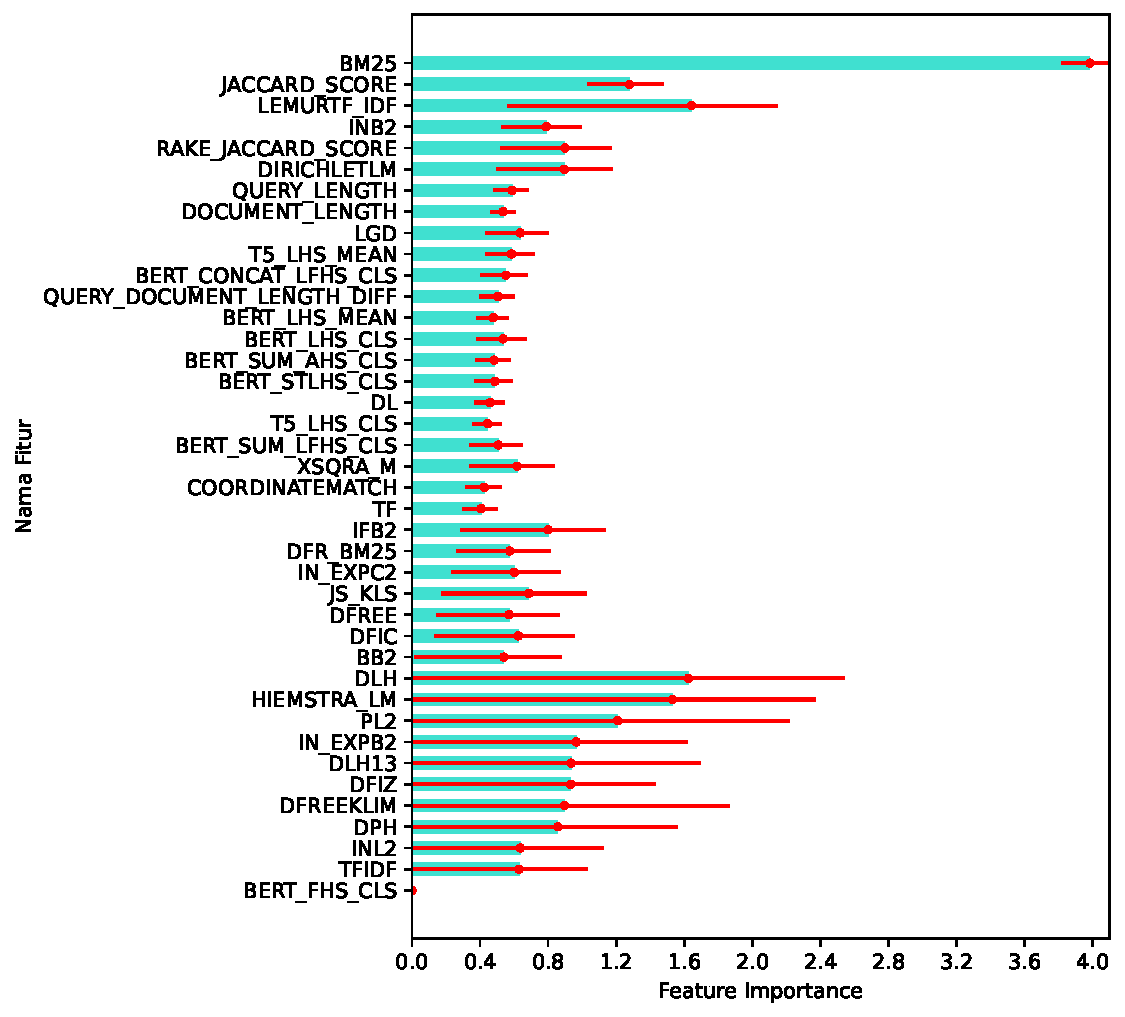
\includegraphics[scale=0.725]{assets/pdfs/Feature Importance Distribution Log.pdf}
    \caption{\feature{} \importance{} secara umum. Perhatikan bahwa sumbu-x merupakan nilai \feature{} \importance{} dalam skala logaritmik, Sementara itu, sumbu-y merupakan daftar nama fitur yang diusulkan terurut secara menurun dari yang paling penting.}
    \label{grafik:Feature Importance All}
\end{figure}
Perlu diketahui bahwa nilai dari \feature{} \importance{} $fi$ yang diperoleh berada dalam interval tertutup $fi\in[0,1]$ dengan nilai $fi=1$ berarti bahwa model hanya menggunakan satu fitur tersebut untuk melakukan seluruh \textit{split}, sedangkan $fi=0$ berarti bahwa fitur tersebut tidak digunakan dalam membuat \textit{split} sama sekali. Namun, sebelum divisualisasikan, karena nilai $fi$ yang diperoleh sangat \textit{skew} sehingga dinormalisasi terlebih dahulu dengan menggunakan $\log(fi \times 100)$. Perhatikan bahwa, karena nilai $fi$ masuk dalam interval tertutup $[0,1]$, maka hasil normalisasi menggunakan fungsi $\log$ akan membuat grafik semakin \textit{skew}, sehingga ditetapkan konstanta pengali $100$ untuk merubah nilai menjadi interval $[0,100]$.

Berdasarkan hasil yang didapat, ditemukan bahwa, secara rata-rata, lima fitur yang paling bermanfaat secara terurut dari yang paling penting adalah \obm{}, LEMURTF\_IDF, DLH, HIEMSTRA\_LM, dan JACCARD\_SCORE. Namun, dari kelima fitur tersebut, dua diantaranya memiliki standar deviasi tinggi, yaitu DLH dan HIEMSTRA\_LM, hal tersebut mencerminkan bahwa dari semua model \lambdamart{} yang dilatih, kedua fitur tersebut tidak konsisten menjadi fitur yang paling penting. Sementara itu, fitur-fitur seperti \obm{}, LEMURTF\_IDF, dan JACCARD\_SCORE menunjukkan hasil yang lebih konsisten dari seluruh model yang dilatih.

Kemudian, seperti yang telah diusulkan pada \subbab{}~\ref{subbab:3:Usulan Fitur}, digunakan juga fitur-fitur yang memanfaatkan keluaran \encoder{}. Untuk metode pemanfaatan vektor \encoder{} \bert{}, ditemukan bahwa CONCAT\_LFHS\_CLS, sama dengan temuan \citet{devlin2018bert}, merupakan fitur yang paling efektif dalam melakukan klasifikasi menurut nilai \importance{}-nya yang relatif lebih tinggi dibanding metode pemanfaatan vektor \bert{} lainnya. Selain itu, untuk metode pengambilan lainnya, ditemukan bahwa urutan nilai \importance{} yang didapat sama dengan urutan efektivitas temuan \citet{devlin2018bert}, dengan pengecualian LHS\_CLS. Hasil eksperimen menunjukkan bahwa LHS\_CLS merupakan fitur kedua yang paling efektif diantara metode pengambilan vektor \bert{} lainnya, bertentangan dengan \citet{devlin2018bert} yang mendapatkan LHS\_CLS sebagai metode terburuk kedua. Sementara itu, untuk metode pemanfaatan \encoder{} \tfive{} didapatkan bahwa hasil eksperimen sesuai dengan temuan \citet{ni2021sentence} dengan LHS\_MEAN sebagai fitur paling efektif. Dari semua metode pengambilan vektor yang diuji, didapat bahwa penggunaan rata-rata dari vektor \hs{} \tfive{} merupakan yang paling efektif, namun nilai \importance{}-nya masih kalah dengan algoritma sederhana seperti JACCARD\_SCORE.

Berdasarkan hasil analisis \feature{} \importance{} tersebut, dilakukan pengujian efektivitas menggunakan data \testing{}. Dibentuk sistem yang sama dengan perbedaan pada jumlah fitur yang diekstraksi, yaitu dengan hanya mengekstraksi fitur nilai relevansi \obm{}, nilai relevansi LemurTF\_IDF, dan nilai kesamaan jaccard. Hasil percobaan tersebut diberikan pada \tabel{}~\ref{tabel:hasil test 3 fitur}. Menurut hasil percobaan, didapatkan bahwa, untuk metrik tolok ukur utama \recall{}$@3$, kinerja sistem relatif naik dengan penambahan proses \reranking{} menggunakan ketiga fitur tersebut. Selain metrik \recall{}$@3$, ditemukan peningkatan pada metrik \precision{}$@3$ yang mengindikasikan bahwa \reranking{} yang dilakukan dapat meningkatkan kualitas tiga dokumen teratas secara efektif.
\begin{table}[H]
    \centering
    \caption{Hasil eksperimen pada data \testing{} menggunakan \reranker{} dengan masukan nilai relevansi \obm{} dan LemurTF\_IDF, serta JACCARD\_SCORE yang diurutkan berdasarkan metrik \recall{}@3}
    \label{tabel:hasil test 3 fitur}
    \resizebox{\textwidth}{!}{%
        \begin{tabular}{lrrrrrrrrr}
	\toprule
	name & R@3 & R@5 & R@10 & recip\_rank & P@3 & P@5 & P@10 & map & nDCG@5 \\
	\midrule
	DLH13 (Reranker) & \textbf{0,7277} & 0,7723 & \underline{0,8614} & 0,7093 & \textbf{0,2871} & 0,1881 & \underline{0,1059} & 0,6613 & 0,6884 \\
	TF\_IDF (Reranker) & \underline{0,7228} & 0,7673 & \underline{0,8614} & 0,7101 & \underline{0,2838} & 0,1861 & \underline{0,1059} & 0,6585 & 0,6839 \\
	BM25 (Reranker) & 0,7129 & \underline{0,7871} & \textbf{0,8663} & 0,7036 & 0,2805 & \textbf{0,1921} & \textbf{0,1069} & 0,6574 & 0,6898 \\
	DLH13 & 0,7129 & \underline{0,7871} & \underline{0,8614} & \textbf{0,7345} & \underline{0,2838} & \underline{0,1901} & \underline{0,1059} & \textbf{0,6813} & \textbf{0,7082} \\
	InL2 (Reranker) & 0,7129 & 0,7822 & 0,8515 & 0,7040 & 0,2805 & 0,1881 & 0,1040 & 0,6561 & 0,6874 \\
	DFR\_BM25 (Reranker) & 0,7079 & \textbf{0,7921} & \textbf{0,8663} & 0,6995 & 0,2772 & \textbf{0,1921} & \textbf{0,1069} & 0,6521 & 0,6880 \\
	BM25 & 0,6881 & \underline{0,7871} & \underline{0,8614} & 0,7147 & 0,2739 & \underline{0,1901} & \underline{0,1059} & 0,6568 & 0,6919 \\
	InL2 & 0,6881 & \underline{0,7871} & \underline{0,8614} & \underline{0,7201} & 0,2706 & \underline{0,1901} & \underline{0,1059} & \underline{0,6693} & \underline{0,6997} \\
	TF\_IDF & 0,6881 & \underline{0,7871} & \underline{0,8614} & 0,7200 & 0,2706 & \underline{0,1901} & \underline{0,1059} & 0,6652 & 0,6975 \\
	DFR\_BM25 & 0,6782 & \underline{0,7871} & 0,8564 & 0,7126 & 0,2706 & \underline{0,1901} & 0,1050 & 0,6573 & 0,6919 \\
	\bottomrule
	\end{tabular}%
    }
\end{table}

Namun, kasus yang sama tidak bisa digeneralisasikan untuk metrik lainnya, seperti yang didapatkan bahwa terjadi penurunan kinerja sistem menurut beberapa metrik. Perubahan nilai metrik diberikan dalam \tabel{}~\ref{tabel:hasil test persentase kenaikan}. Perhatikan bahwa, walaupun didapatkan peningkatan pada \recall{}$@3$, terdapat penurunan nilai metrik untuk \recall{}$@5$ atau \recall{}$@10$. Hal tersebut menunjukkan bahwa secara rata-rata penambahan \reranker{} dengan tiga fitur tersebut dapat meningkatkan kemampuan sistem untuk mengidentifikasi dokumen relevan pada tiga hasil teratas. Tetapi, selain tiga hasil teratas, relevansi yang didapatkan kurang lebih sama atau bahkan menurun, yang berarti sistem tidak efektif dalam mempertahankan relevansi untuk cakupan yang lebih luas.

\begin{table}[H]
    \centering
    \caption{Persentase perubahan metrik pada data \testing{}}
    \label{tabel:hasil test persentase kenaikan}
    \resizebox{\textwidth}{!}{%
        \begin{tabular}{lrrrrrrrrr}
	\toprule
	name & R@3 & R@5 & R@10 & recip\_rank & P@3 & P@5 & P@10 & map & nDCG@5 \\
	\midrule
	TF\_IDF (Reranker) & \textbf{5,036}\% & -2,516\% & 0,000\% & \textbf{-1,375}\% & \textbf{4,878}\% & -2,083\% & 0,000\% & -1,000\% & -1,950\% \\
	DFR\_BM25 (Reranker) & \underline{4,380}\% & \textbf{0,629}\% & \textbf{1,156}\% & -1,850\% & 2,439\% & \textbf{1,042}\% & \textbf{1,887}\% & \underline{-0,793}\% & \underline{-0,575}\% \\
	BM25 (Reranker) & 3,597\% & \underline{0,000}\% & \underline{0,575}\% & \underline{-1,553}\% & 2,410\% & \textbf{1,042}\% & \underline{0,935}\% & \textbf{0,095}\% & \textbf{-0,299}\% \\
	InL2 (Reranker) & 3,597\% & -0,629\% & -1,149\% & -2,226\% & \underline{3,659}\% & \underline{-1,042}\% & -1,869\% & -1,963\% & -1,767\% \\
	DLH13 (Reranker) & 2,083\% & -1,887\% & 0,000\% & -3,439\% & 1,163\% & \underline{-1,042}\% & 0,000\% & -2,929\% & -2,800\% \\
        \hline
        \textit{mean} & 3,739\% & -0,881\% & 0,116\% & -2,089\% & 2,910\% & -0,417\% & 0,190\% & -1,318\% & -1,478\% \\
	\bottomrule
	\end{tabular}%
    }
\end{table}

Sama seperti analisis sebelumnya, dilakukan perhitungan \textit{t-test} untuk mendapatkan signifikansi dari dampak tersebut. Dapat dilihat pada \tabel{}~\ref{tabel:hasil test ttest} yang menunjukkan nilai \textit{p-value} untuk setiap metrik yang diperoleh pada pengujian menggunakan data \testing{}. Menurut hasil tersebut, penambahan proses \reranking{} yang memanfaatkan \reranker{} berbasis fitur dengan tiga fitur masukan tersebut tidak memiliki dampak signifikan untuk setiap metrik. Oleh karena itu, menurut metrik utama \recall{}$@3$, dapat disimpulkan bahwa \reranking{} menggunakan ketiga fitur tersebut dapat meningkatkan performa sistem \ir{} sekitar $3,739\%$ namun tidak cukup signifikan.
\begin{table}[H]
    \centering
    \caption{Hasil \textit{t-test} eksperimen pada data \testing{}}
    \label{tabel:hasil test ttest}
    \resizebox{\textwidth}{!}{%
        \begin{tabular}{lrrrrrrrrr}
	\toprule
        \multirow{2}{*}{name} & \multicolumn{9}{c}{\textit{p-value}} \\ \cline{2-10}
        & R@3 & R@5 & R@10 & recip\_rank  & P@3 & P@5 & P@10 & map & nDCG@5 \\
	\midrule
	BM25 (Reranker) & 0,4376 & 1,0000 & 0,7647 & 0,6433 & 0,5955 & 0,7831 & 0,6570 & 0,9777 & 0,9243 \\
	DFR\_BM25 (Reranker) & 0,3453 & 0,8737 & 0,6195 & 0,5879 & 0,6195 & 0,7977 & 0,5298 & 0,8197 & 0,8597 \\
	DLH13 (Reranker) & 0,5800 & 0,5925 & 1,0000 & 0,3101 & 0,7647 & 0,7831 & 1,0000 & 0,3733 & 0,3680 \\
	InL2 (Reranker) & 0,3557 & 0,8628 & 0,5298 & 0,5194 & 0,3683 & 0,7977 & 0,3197 & 0,5766 & 0,5839 \\
	TF\_IDF (Reranker) & 0,2248 & 0,4680 & 1,0000 & 0,6675 & 0,2502 & 0,5663 & 1,0000 & 0,7641 & 0,5357 \\
	\bottomrule
	\end{tabular}%
    }
\end{table}
%-----------------------------------------------------------------------------%





%-----------------------------------------------------------------------------%
\subsection{Hasil Pengaruh \Cutoff{}}
\label{subbab:5::Hasil Pengaruh Cut-off}
Pada \gambar{}~\ref{grafik:cutoff} diberikan hasil eksperimen untuk metrik \recall{} pada \cutoff{} 3. Namun, grafik tersebut kurang dapat menunjukkan korelasi antara \cutoff{} dengan efektivitas. Dapat dilihat bahwa sistem DLH13 (Reranker) memiliki hasil yang paling baik pada \cutoff{} 85, sedangkan efektivitas kedua terbaik didapatkan oleh sistem TF\_IDF pada \cutoff{} 150. Oleh karena itu, berdasarkan hasil eksperimen, kurang adanya bukti yang dapat mendukung hipotesis awal peneliti, yaitu terdapat korelasi positif antara nilai \cutoff{} dengan kinerja sistem.
\begin{landscape}
    \begin{figure}
        \centering
        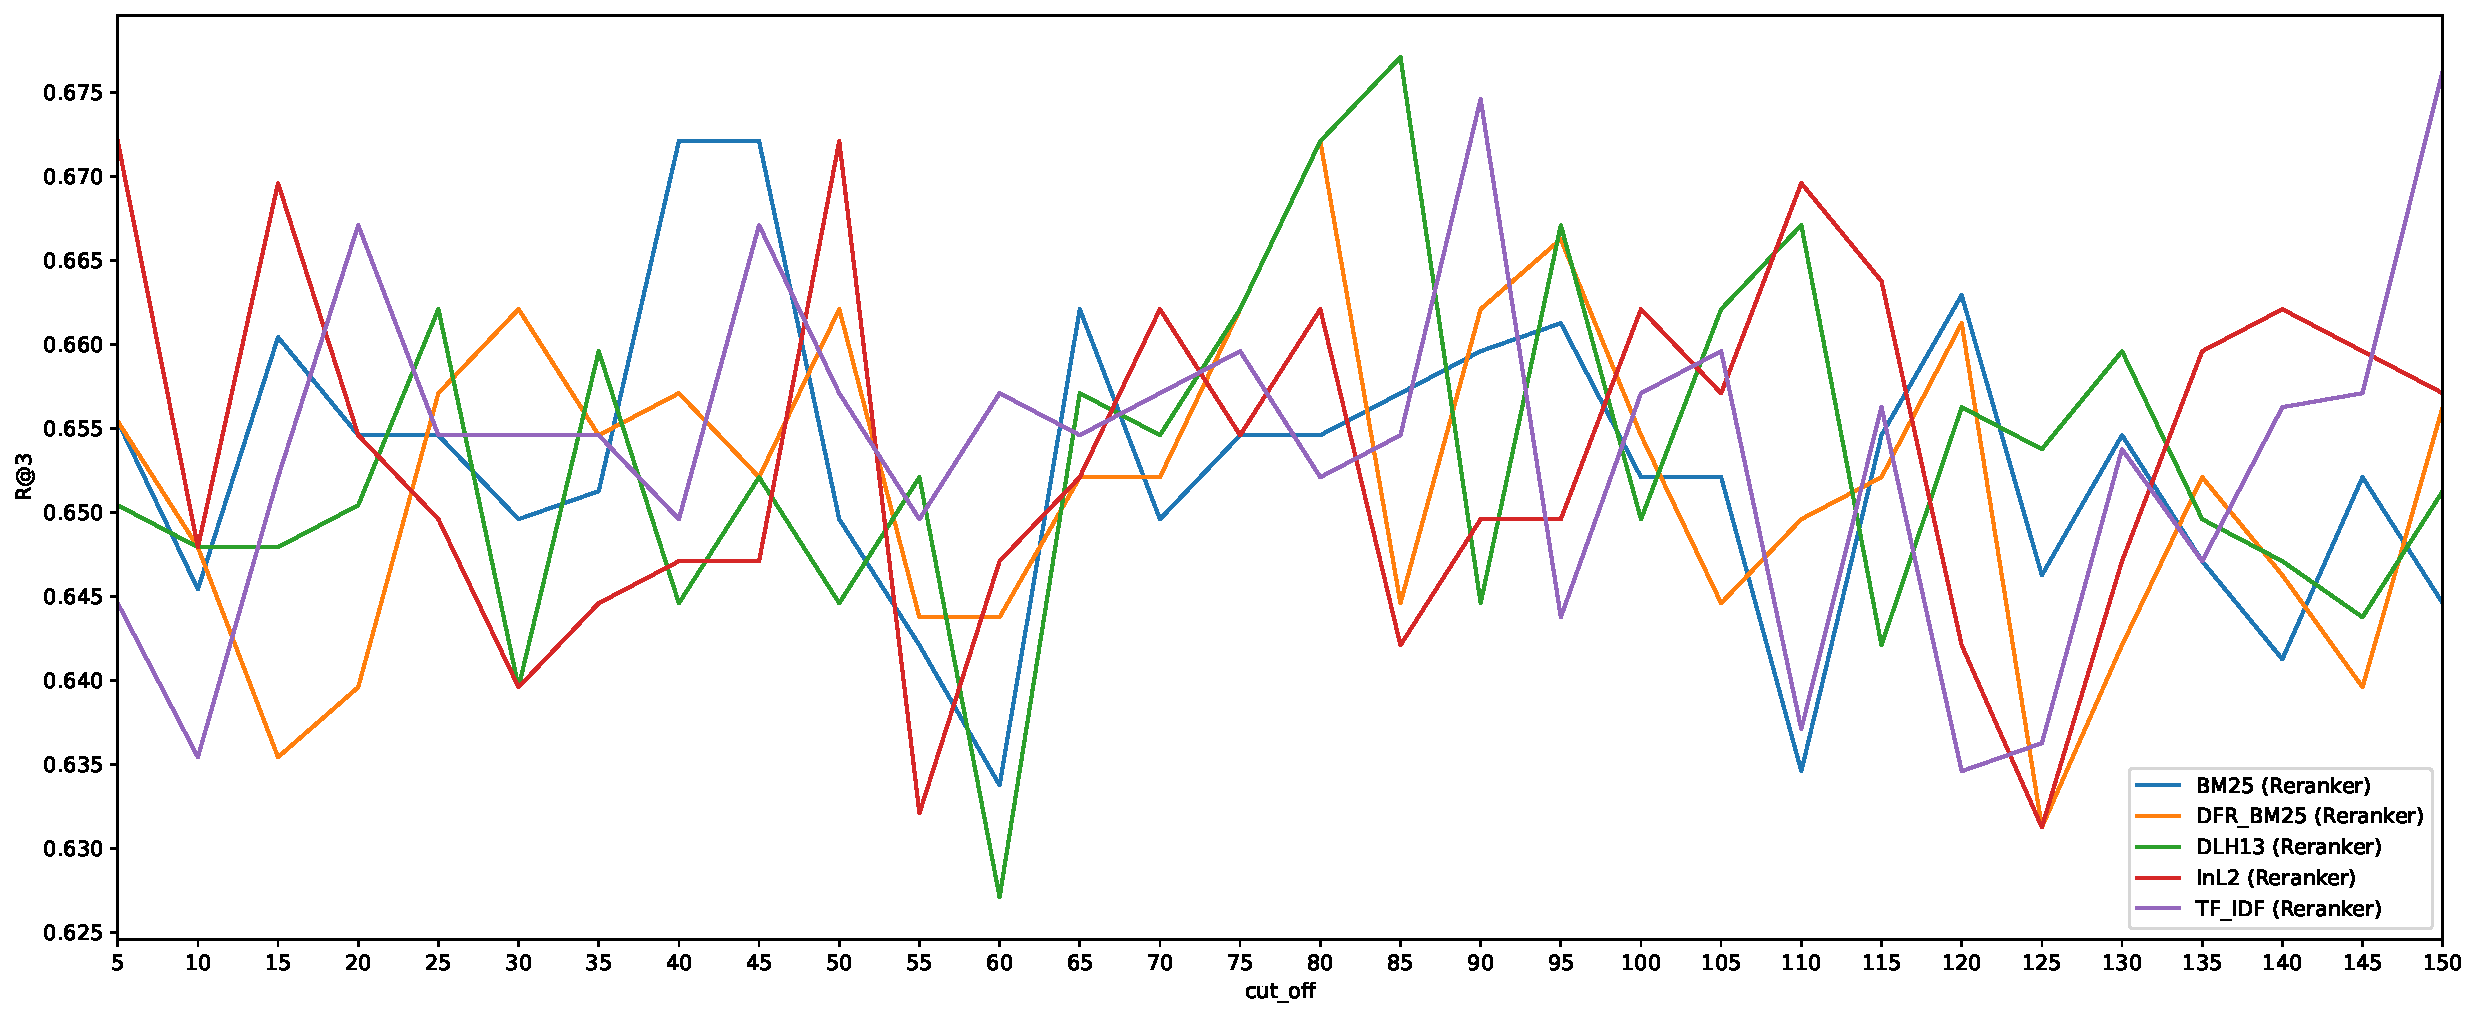
\includegraphics[scale=0.6]{assets/pdfs/Cut Off Experiment Results_3.pdf}
        \caption{Kinerja pada beberapa \cutoff{}. Perhatikan bahwa tidak didapatkannya korelasi yang kuat dengan nilai \textit{pearson} sebagai berikut: BM25 (Reranker) -0.2363; DFR\_BM25 (Reranker) -0.0904; DLH13 (Reranker) 0.1239; InL2 (Reranker) 0.0277; dan TF\_IDF (Reranker) 0.046. Hasil tersebut menunjukkan bahwa BM25 (Reranker) memiliki korelasi negatif yang sangat lemah dan DFR\_BM25 (Reranker) memiliki korelasi negatif yang lemah, serta DLH13 (Reranker), InL2 (Reranker), dan TF\_IDF (Reranker) memiliki korelasi positif yang lemah. Oleh karena itu, kurang adanya bukti yang mendukung hipotesis bahwa terdapat korelasi positif antara nilai \cutoff{} dengan kinerja sistem.}
        \label{grafik:cutoff}
    \end{figure}
\end{landscape}
%-----------------------------------------------------------------------------%





%-----------------------------------------------------------------------------%
\section{Rangkuman Hasil Eksperimen}
\label{subbab:5:Rangkuman Hasil Eksperimen}
% \todo{FEATURE IMPORTANCE BEST ONES\\FEATURE IMPORTANCE ENCODER EMBEDDING X CHK\\PERFORMANCE VAL\\SIGNIFICANCE VAL\\PERFORMANCE TEST WITH SELECTED FEATURES\\SIGNIFICANCE TEST WITH SELECTED FEATURES\\CUT-OFF CORRELATION\\HYPOTHESIS CORRELATION}

Berdasarkan hasil eksperimen, didapat bahwa penambahan \lambdamart{} sebagai \reranker{} dengan menggunakan seluruh fitur usulan dapat mengingkatkan seluruh metrik sekitar $4,17\%$ dan $4,19\%$ untuk metrik utama secara signifikan. Terdapat tiga sistem yang ditemukan memiliki performa terbaik berdasarkan kasus tertentu. Pertama, DLH13 (Reranker) merupakan sistem terbaik untuk melakukan pengembalian dokumen pada 3 hasil teratas yang diindikasikan dengan metrik \recall{}$@3$ dan \precision{}$@3$ tertinggi diantara kelima sistem tersebut. Namun, untuk cakupan dokumen yang lebih luas, TF\_IDF (Reranker) dapat dijadikan alternatif karena mendapatkan metrik \recall{}$@10$ dan \precision{}$@10$ tertinggi dibandingkan sistem lainnya. Sementara itu, DFR\_BM25 (Reranker) merupakan hasil yang baik dibandingkan dengan sistem lainnya dalam kasus tertentu yang memerlukan ketepatan pengembalian pada dokumen-dokumen teratas dibandingkan jumlah relevansi yang dikembalikan.

Kemudian, dari hasil analisis \feature{} \importance{}, terdapat tiga fitur yang penting untuk melakukan penilaian relevansi dokumen, yaitu nilai relevansi dari \obm{} dan LEMURTF\_IDF, serta nilai kesamaan jaccard antara himpunan kata dokumen dan kueri. Dengan hanya ketiga fitur tersebut, diuji performa sistem pada data \testing{}. Hasil menunjukkan peningkatan pada \recall{}$@3$ dan \precision{}$@3$, namun tidak sepenuhnya membaik untuk metrik lainnya. Oleh karena itu, dapat disimpulkan bahwa, berdasarkan metrik utama, ketiga fitur tersebut dapat meningkatkan kinerja sekitar $3,739\%$ namun belum cukup signifikan. Selain itu, ditemukan bahwa \importance{} fitur \encoder{} serupa dengan performa temuan penelitian sebelumnya~\citep{devlin2018bert, ni2021sentence}, namun kurang bermanfaat untuk menentukan relevansi dokumen legal, melihat bahwa fitur tersebut memiliki \importance{} yang lebih kecil dibandingkan perhitungan kesamaan sederhana seperti jaccard.

Sementara itu, berdasarkan pengamatan, tidak ditemukan korelasi antara \cutoff{} dan efektivitas untuk rentang \cutoff{} dari 5 sampai 150 dengan interval 5. Namun, menurut nilai perhitungan korelasi \textit{pearson}, ditemukan korelasi positif sangat lemah untuk sistem DLH13 (Reranker), InL2 (Reranker), dan TF\_IDF (Reranker). Sementara itu, terdapat korelasi negatif lemah untuk sistem DFR\_BM25 (Reranker) dan korelasi negatif sangat lemah untuk sistem BM25 (Reranker). Hal tersebut bertentangan dengan hipotesis awal bahwa semakin banyak dokumen yang dikembalikan maka \lambdamart{} dapat melakukan lebih banyak pertimbangan yang dapat semakin meningkatkan kinerja sistem.
%-----------------------------------------------------------------------------%





%-----------------------------------------------------------------------------%
% \begin{figure}
%     \centering
%     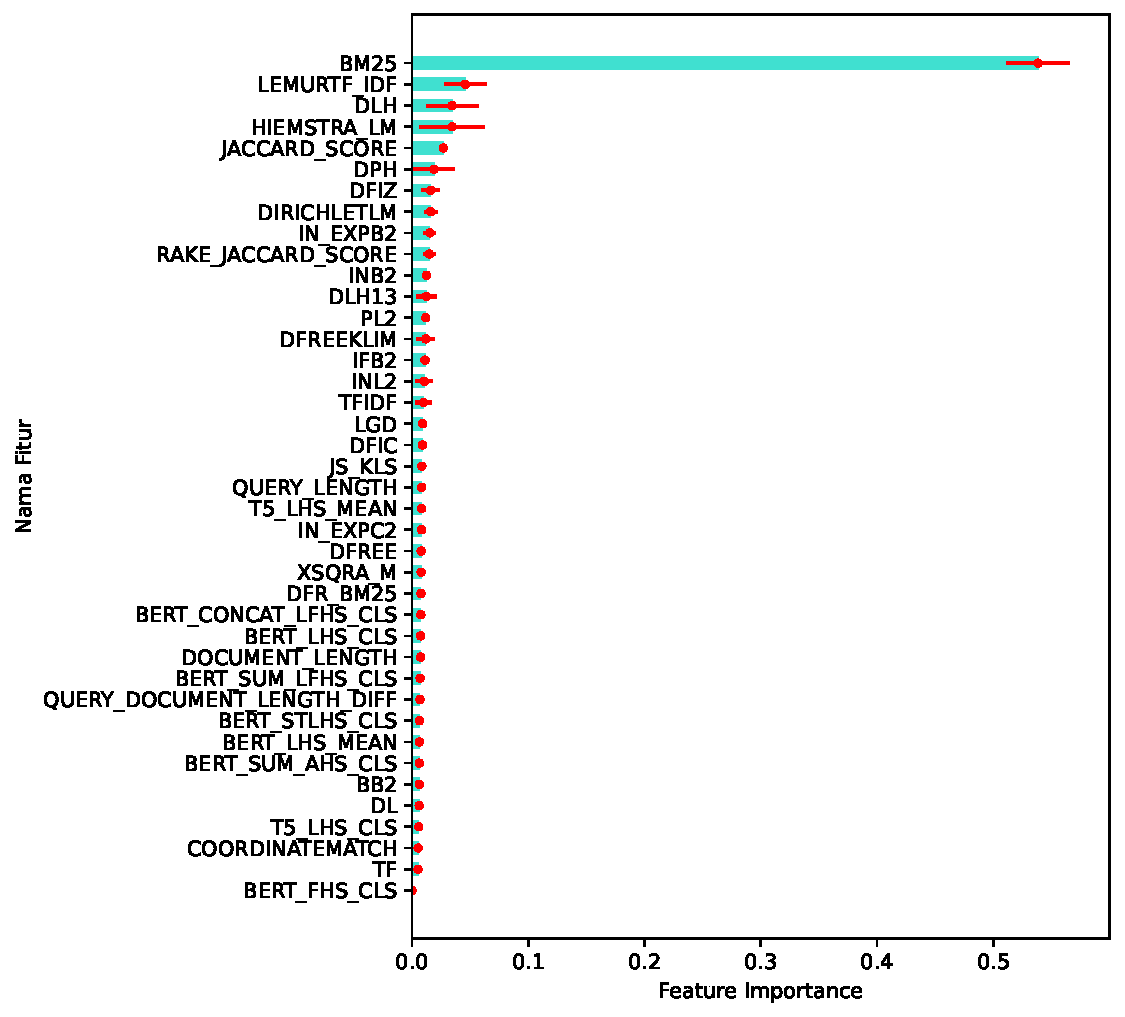
\includegraphics[scale=0.65]{assets/pdfs/Feature Importance BM25.pdf}
%     \caption{Feature Importance BM25 (Reranker)}
%     \label{grafik:Feature Importance BM25 All}
% \end{figure}

% \begin{figure}
%     \centering
%     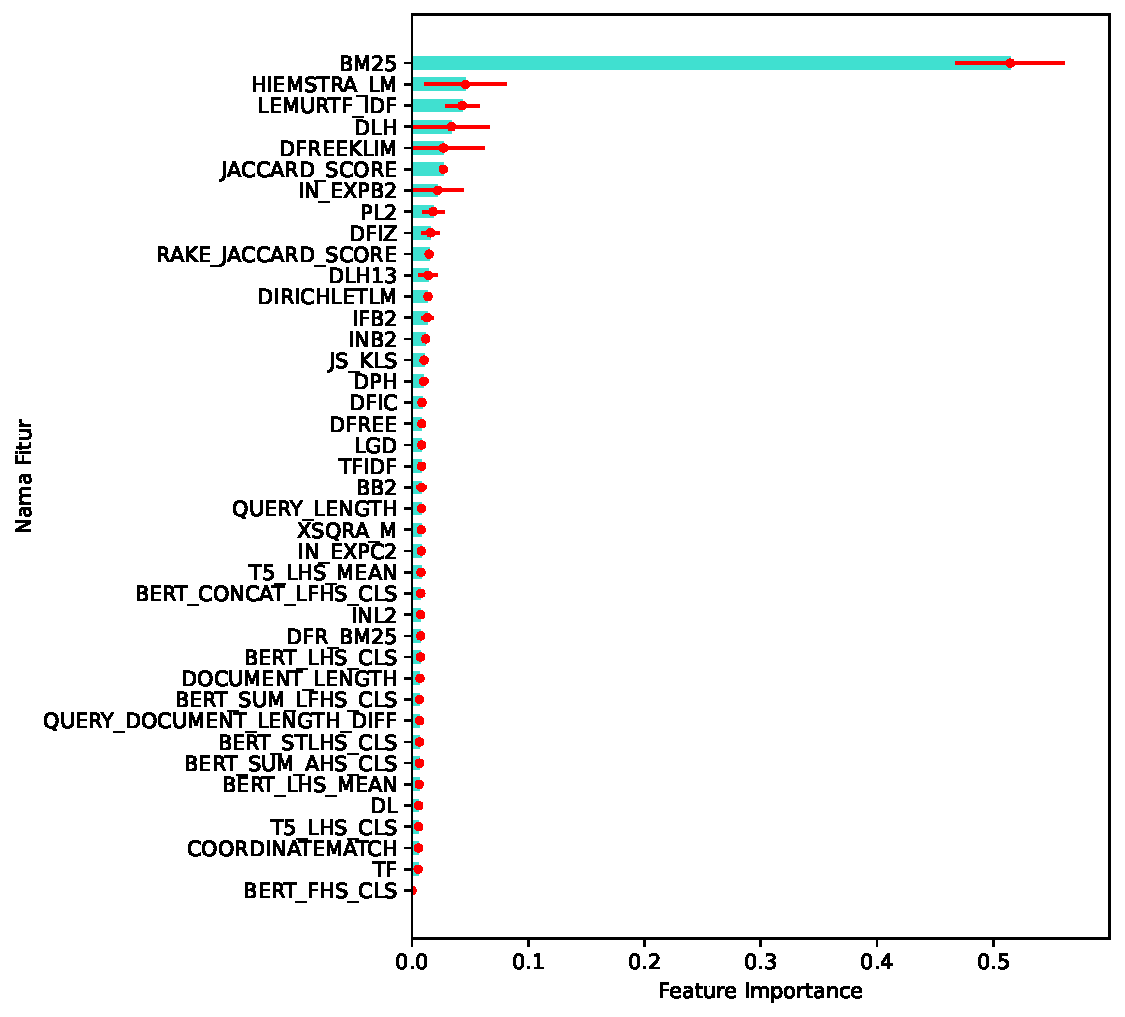
\includegraphics[scale=0.65]{assets/pdfs/Feature Importance TF_IDF.pdf}
%     \caption{Feature Importance TF\_IDF (Reranker)}
%     \label{grafik:Feature Importance TF_IDF All}
% \end{figure}

% \begin{figure}
%     \centering
%     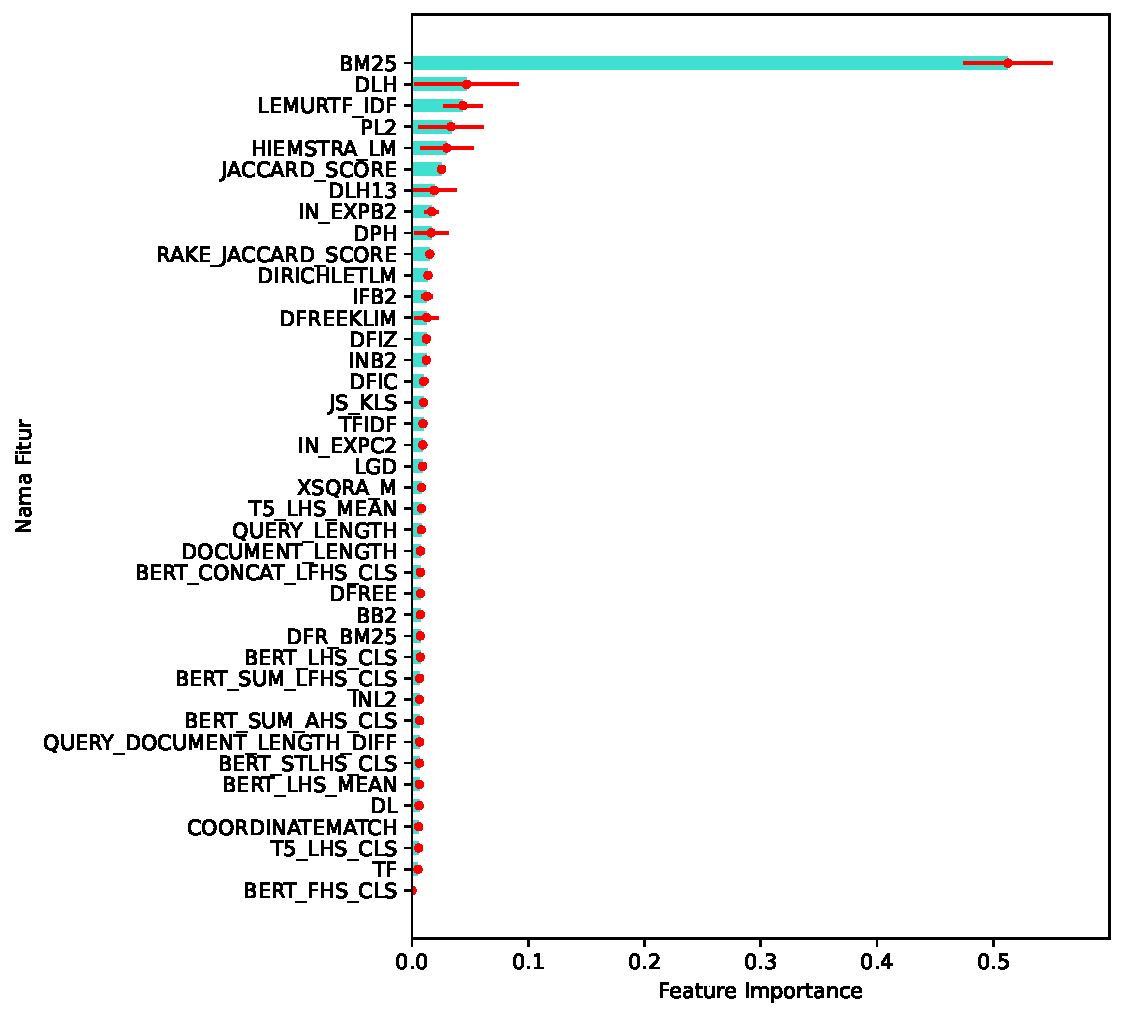
\includegraphics[scale=0.65]{assets/pdfs/Feature Importance InL2.pdf}
%     \caption{Feature Importance InL2 (Reranker)}
%     \label{grafik:Feature Importance InL2 All}
% \end{figure}

% \begin{figure}
%     \centering
%     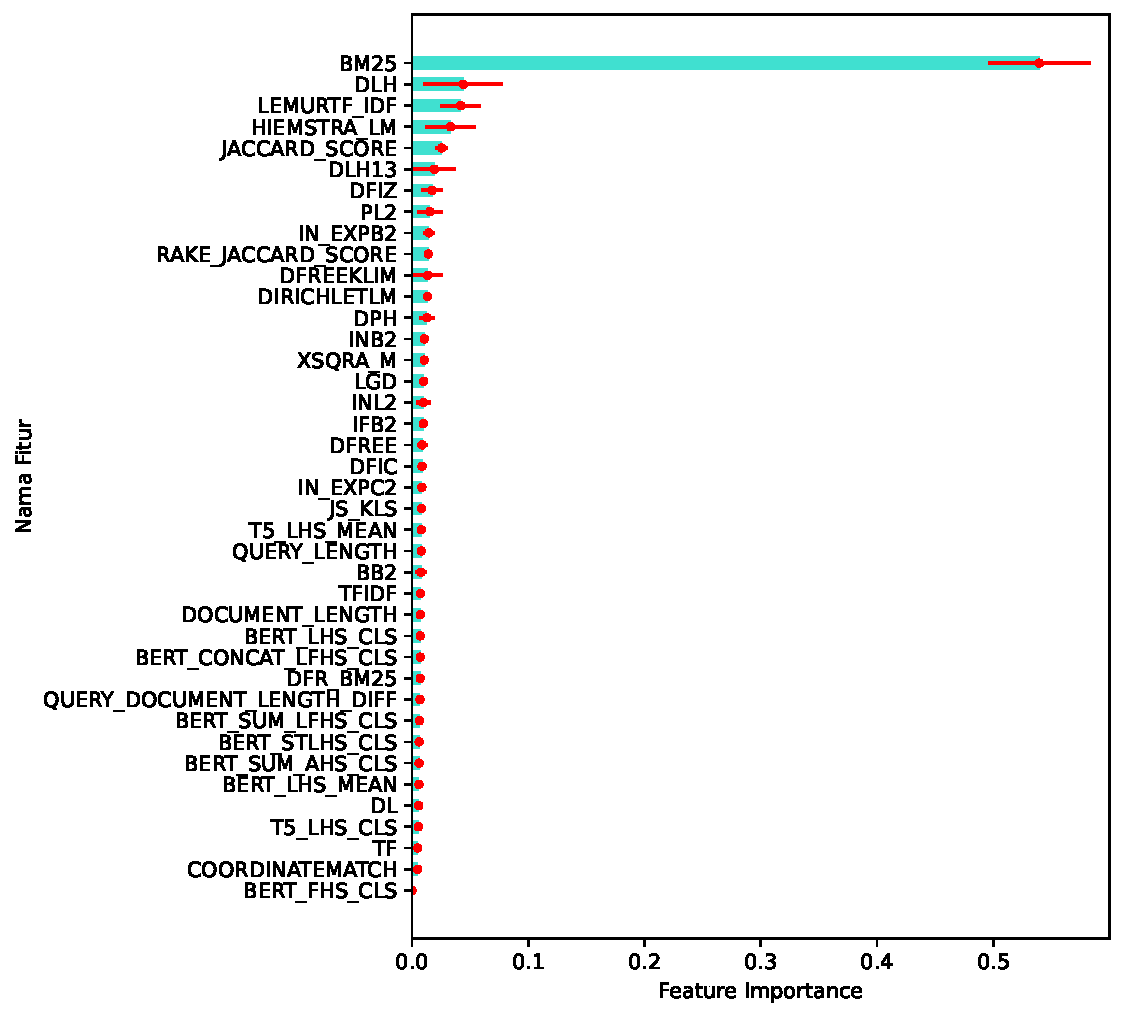
\includegraphics[scale=0.65]{assets/pdfs/Feature Importance DFR_BM25.pdf}
%     \caption{Feature Importance DFR\_BM25 (Reranker)}
%     \label{grafik:Feature Importance DFR_BM25 All}
% \end{figure}

% \begin{figure}
%     \centering
%     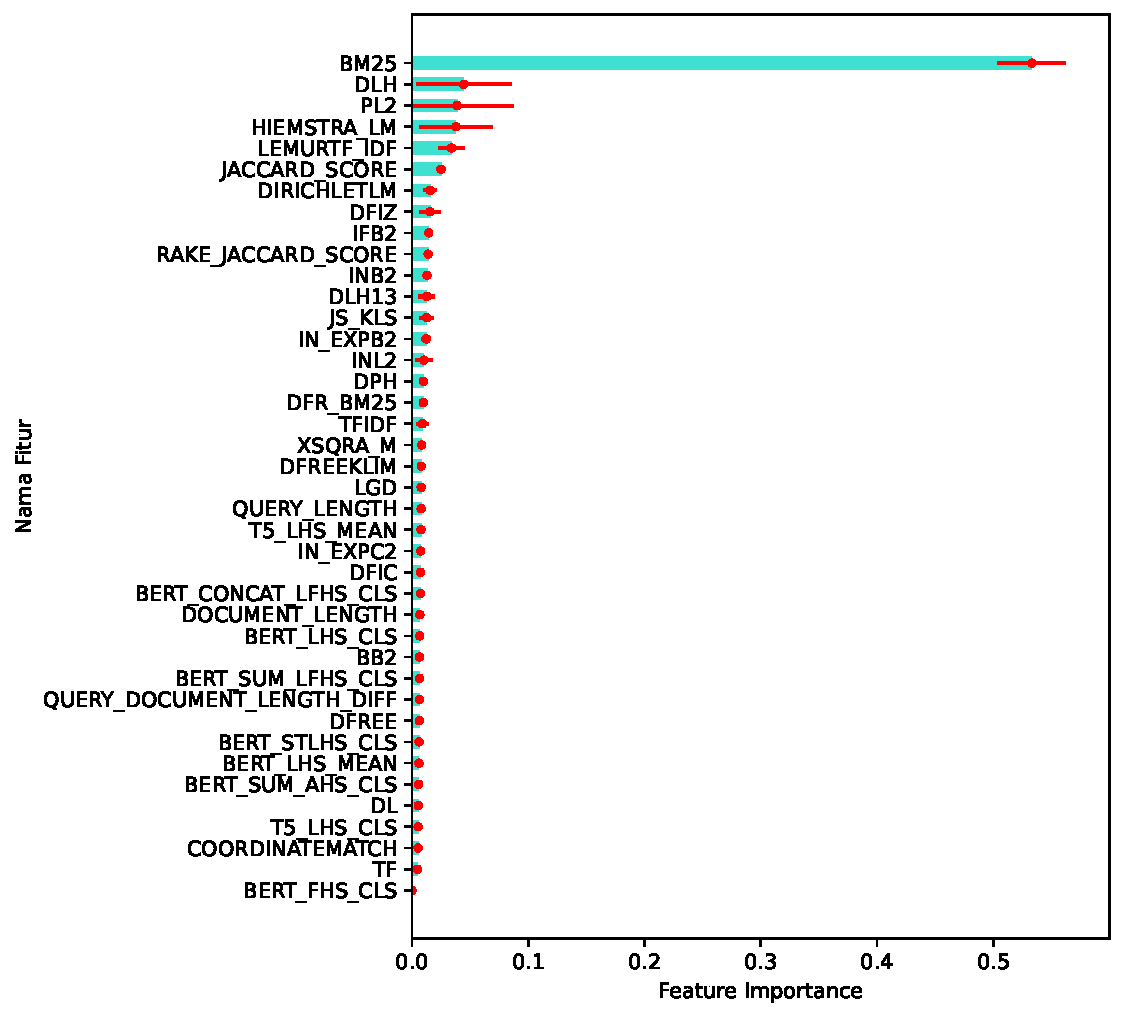
\includegraphics[scale=0.65]{assets/pdfs/Feature Importance DLH13.pdf}
%     \caption{Feature Importance DLH13 (Reranker)}
%     \label{grafik:Feature Importance DLH13 All}
% \end{figure}
%-----------------------------------------------------------------------------%